\documentclass{article}
\usepackage{customized_arxiv}

\usepackage[utf8]{inputenc}
\usepackage[english, russian]{babel}
\usepackage[T1]{fontenc}
\usepackage{url}
\usepackage{booktabs}
\usepackage{amsfonts}
\usepackage{nicefrac}
\usepackage{microtype}
\usepackage{lipsum}
\usepackage{graphicx}
\usepackage{natbib}
\usepackage{doi}
\usepackage{amsmath, amsfonts, amssymb, amsthm, mathtools}
\usepackage{algorithm}
\usepackage{algpseudocode}
\theoremstyle{definition}
\newtheorem{definition}{Definition}
\theoremstyle{assumption}
\newtheorem{assumption}{Assumption}
\theoremstyle{lemma}
\newtheorem{lemma}{Lemma}
\theoremstyle{theorem}
\newtheorem{theorem}{Theorem}
\theoremstyle{proposition}
\newtheorem{proposition}{Proposition}


\title{Стохастический метод Ньютона с различным семплингом}
\author{Денис Швейкин
	%% examples of more authors
	\And
	Рустем Исламов
	%% \AND
	%% Coauthor \\
	%% Affiliation \\
	%% Address \\
	%% \texttt{email} \\
	%% \And
	%% Coauthor \\
	%% Affiliation \\
	%% Address \\
	%% \texttt{email} \\
	%% \And
	%% Coauthor \\
	%% Affiliation \\
	%% Address \\
	%% \texttt{email} \\
}
\date{}

\renewcommand{\shorttitle}{Стохастический метод Ньютона с различным семплингом}

%%% Add PDF metadata to help others organize their library
%%% Once the PDF is generated, you can check the metadata with
%%% $ pdfinfo template.pdf
\hypersetup{
	pdftitle={Стохастический метод Ньютона с различным семплингом},
	pdfsubject={},
	pdfauthor={Денис Швейкин, Рустем Исламов},
	pdfkeywords={},
}

\begin{document}
	
	\maketitle
	
	\begin{abstract}
		
		Задача минимизации среднего от большого числа гладких сильно выпуклых функций встречается в машинном обучении повсеместно. Стохастические методы первого порядка, такие как стохастический градиентный спуск (SGD), для этой задачи хорошо изучены. В свою очередь, методы второго порядка, такие как метод Ньютона имеют определенные преимущества, поскольку могут адаптироваться к кривизне задачи. Также они известны своей быстрой сходимостью. Однако стохастические варианты методов типа Ньютон изучены не так хорошо, как методы типа SGD, и имеют ограничения на размеры батчей. Ранее был предложен метод, который не требует таких ограничений. Наша работа исследует этот метод с различными стратегиями семплинга, которые ведут практическим улучшениям.
		
	\end{abstract}
	
	
	\keywords{Стохастический метод Ньютона, стратегии семплинга}
	
	\section{Introduction}
	
	The problem is to minimize the empirical risk which has finite-sum structure \cite{kovalev2019stochastic}:
	\begin{equation}\label{ERM}
		\underset{x \in \mathbb R^d}{\min} \left[ f(x) \overset{def}{=} \frac{1}{n} \sum \limits_{i=1}^n f_i(x) \right],
	\end{equation}
	where each $f_i$ is assumed to have Lipschitz Hessian. 
	
	Typically, $n$ - the total number of functions - is very large for modern real-world problems. Thus, the stochastic approach is used because it is computationally difficult to evaluate the gradient of all $f_i$ at each step. The Stochastic Gradient Descent (SGD) method \cite{SGD-1} calculates the gradients of some randomly chosen $f_i$ which leads to cheaper computation per-iteration cost compared to the vanilla Gradient Descent (GD). The analysis of SGD and its modifications is rich and well explored. Firstly, the theory of SGD-type methods does not restrict the batch size. Therefore, these algorithms can be applied even with small batches. It is known that simple SGD converges only to a neighbourhood of the solution only \cite{sgd-hogwild, sgd-general-analysis} whose size is proportional to the variance of the stochastic gradient. However, there are techniques (also known as variance reduction) to solve this issue. These techniques \cite{exp-convergence, advances-NIPS, unified-sgd, one-method} modify the update rule of vanilla SGD which allows to mitigate the aforementioned effect without changing per-iteration cost. However, the main disadvantage of all gradient-type methods is that a computation complexity depends on the curvature of the problem, which is called the condition number and is defined as the ratio of Lipschitzness and strong convexity parameters. 
	
	This is a place where second-order methods such as the Newton method \cite{Nesterov-introductory, Newton-convergence, RSN} come to play. Taking into account second-order derivatives it possible to adjust the algorithm's step sizes to the curvature of the problem \cite{Nesterov-introductory}. Unfortunately, much less work has been done in the direction of stochastic Newton-type methods. Many methods \cite{sub-sampled, exact-inexact, variance-reduced-Newton, zhang2022adaptive, tripuraneni2018stochastic, zhou2020stochastic} require large batch sizes. In particular, the required batch size is commonly quadratically proportional to the inverse of the desired accuracy. That means that one need to evaluate a large number of $f_i$ Hessians which sometimes can be much larger than $n$. \cite{kovalev2019stochastic} proposes a simple Stochastic Newton algorithm, which can work with batches of any size. This algorithm achieves local linear and in come cases super-linear convergence rates. 
	
	In practice, various sampling strategies are used for SGD-type algorithms to improve further the performance. One of the most famous sampling mechanisms is so-called Importance Sampling \cite{gower2019sgd, https://doi.org/10.48550/arxiv.1401.2753, 9413313}. The idea is to compute gradients of the functions that have more impact on the problem. Another method of random optimization is Random Reshuffling, which does iterative gradient steps passing reshuffled data \cite{mishchenko2020random}. \cite{richtarik2016parallel} studies many other sampling mechanisms. We analyse such strategies, but for the Algorithms $1$ of \cite{kovalev2019stochastic}, to improve the theoretical and practical applications of the algorithms. We explore various sampling strategies supporting them with  rigorously constructed experiments. 
	
	\section{Problem statement}
	
	We consider classical empirical risk minimization (ERM) which typically arises in many machine learning problems to train a model. The objective function $f$ (\ref{ERM}) is an average of a large number of functions $f_i$, where $f_i$ represents a loss on the $i$-th train data point. For example, this notation can be attributed to linear regression. In this case the goal is to find optimal model parameters $x$ that minimize the mean squared error (MSE) on the train data.
	
	\subsection{Assumptions}
	
	We make standard assumptions on functions $f_i$; the same that were originally taken into account in \cite{kovalev2019stochastic}.
	
	
	\begin{assumption}[Strong convexity] A differentiable function $\phi:\ \mathbb R^d \rightarrow \mathbb R$ is $\mu$-strongly convex, where $\mu > 0$, if $\forall\ x, y \in \mathbb R^d$
		
		\begin{equation}\label{strong-conv}
			\phi(x) \geqslant \phi(y) + \langle \nabla \phi, x - y \rangle + \frac{\mu}{2} \| x - y \|^2,
		\end{equation}
	\end{assumption}
	where the norm $\| \cdot \|$ is Euclidean. For twice differentiable functions this assumption is equivalent to the Hessian having each eigenvalue $\geqslant \mu$.
	
	\begin{assumption}[Lipschitz Hessian] A function $\phi: \mathbb R^d \rightarrow R$ has $H$-Lipschitz Hessian if $\forall\ x, y \in \mathbb R^d$
		
		\begin{equation}\label{lip-hess}
			\| \nabla^2 \phi(x) - \nabla^2 \phi(y) \| \leqslant H \| x - y \|
		\end{equation}
	\end{assumption}
	
	\subsection{Sampling}
	
	\begin{definition}[Sampling]
		A random set-valued mapping $\hat S:\ [n] \rightarrow 2^{[n]}$ is called sampling.
	\end{definition}
	
	That means that each $S_k \subseteq [n]$ is a realization of $\hat S$. In this case we can call any probability distribution on $2^{[n]}$ a sampling strategy.
	\subsection{Algorithm}
	
	We apply different sampling strategies on top of the Algorithm 1 from \cite{kovalev2019stochastic}:
	
	\begin{algorithm}
		\caption{Stochastic Newton (SN)}\label{SN}
		\begin{algorithmic}
			\item \textbf{Initialize:} Choose starting iterates $w_1^0, w_2^0, ... w_n^0 \in \mathbb R^d$
			
			\item \For {$k = 0, 1, 2, ...$}	
			
			$ x^{k+1} = \left[ \frac{1}{n} \sum \limits_{i=1}^n \nabla^2 f_i(w_i^k) \right]^{-1} \left[ \frac{1}{n} \sum \limits_{i=1}^n \nabla^2 f_i(w_i^k) w_i^k - \nabla f_i(w_i^k) \right] $
			
			Choose a subset $S^k \subseteq \{ 1, 2, ..., n \}$ with one of the sampling strategies
			
			$w_i^{k+1} = 
			\begin{cases}
				x^{k+1} & i \in S^k \\
				w_i^k & i \notin S^k
			\end{cases}$
			
			\item \EndFor
		\end{algorithmic}
	\end{algorithm}
	
	\subsection{Goal of the project}
	
	We compare different sampling strategies for the Algorithm \ref{SN} proving convergence guarantees and showing practical improvements over the baseline strategy.
	
	
	\section{Theory}	
	
	\subsection{Proofs for the Algorithm}
	
	The convergence of the Algorithm \ref{SN} was clearly described and proven in \cite{kovalev2019stochastic}. Firstly, we look at the statements of three lemmas from the aforementioned article.
	
	\begin{lemma}\label{lemma:1}
		Let $f_i$ be $\mu$-strongly convex and have $H$-Lipschitz Hessian for all $i = 1,...,n$ and consider the following Lyapunov function
		\begin{equation}
			\mathcal W^k \overset{\text{def}} = \frac{1}{n} \sum \limits_{i=1}^n \| w_i^k - x^* \|^2,
		\end{equation}
		where $x^*$ is the minimizer of the objective function $f$ (\ref{ERM}). Then the iterates of the Algorithm \ref{SN} satisfy
		\begin{equation}
			\|x^{k+1} - x^*\| \leqslant \frac{H}{2 \mu} \mathcal W^k.
		\end{equation}
	\end{lemma}
	
	\begin{lemma}\label{lemma:2}
		Assume that every $f_i$ is $\mu$-strongly convex and has $H$-Lipschitz Hessian. If $\|w_i^0 - x^*\| \leqslant \frac{\mu}{H}$ for $i = 1, ..., n$, then for all $k$
		\begin{equation}
			\mathcal W^k \leqslant \frac{\mu^2}{H^2}.
		\end{equation}
	\end{lemma}
	
	The last lemma is the one that incorporates the nature of the sampling strategy. The authors of the Algorithm \ref{SN} used so called $\tau$-nice sampling, which chooses a subset $S^{k} \subseteq \{ 1, 2, ..., n \}$ precisely of size $\tau$ uniformly at random. Therefore it is possible to determine the expectation $\mathbb E_k[\mathcal W^{k+1}] \overset{\text{def}} = \mathbb E[\mathcal W^{k+1} | x^k, w_1^k, ..., w_n^k]$.
	
	\begin{lemma}\label{lemma:3}
		The random iterates of the Algorithm \ref{SN} with $\tau$-nice sampling satisfy the identity
		\begin{equation}
			\mathbb E_k[\mathcal W^{k+1}] = \frac{\tau}{n} \| x^{k+1} - x^* \|^2 + \left(1 - \frac{\tau}{n}\right) \mathcal W^k
		\end{equation}
	\end{lemma}
	
	Then follows the theorem, which estimates the convergence rate of the Algorithm \ref{SN} with $\tau$-nice sampling.
	
	\begin{theorem} \label{theorem:1}
		Assume that every $f_i$ is $\mu$-strongly convex and has $H$-Lipschitz Hessians. Then for the random iterates of the Algorithm 1 we have the recursion
		\begin{equation}
			\mathbb E_k[\mathcal W^{k+1}] \leqslant \left( 1 - \frac{\tau}{n} + \frac{\tau}{n} \left( \frac{H}{2\mu} \right)^2 \mathcal W^k \right) \mathcal W^k.
		\end{equation}
		Moreover, if $\forall i\ \|w_i^0 - x^*\| \leqslant \frac{\mu}{H}$ then
		\begin{equation}
			\mathbb E_k[\mathcal W^{k+1}] \leqslant \left( 1 - \frac{3\tau}{4n} \right) \mathcal W^k.
		\end{equation}
	\end{theorem}
	
	
	\subsection{Sampling Strategies}
	
	\subsubsection{Doubly Uniform Strategies}
	
	To begin with, we discuss the sampling strategies that were presented in \cite{richtarik2016parallel} in relation to the Parallel Coordinate Descend method. These strategies are \textit{Doubly Uniform.}
	
	\begin{definition}[Doubly Uniform (DU) sampling] \label{DU}
		This is a sampling strategy that generates all sets of equal cardinality with equal probability. That is, if $|S_1| = |S_2|$ then $\mathbb P(S_1) = \mathbb P(S_2)$.
	\end{definition}
	
	The name comes from the fact this property is stronger than \textit{uniformity}, which means that all $i \in [n]$ have equal probability to be included in the chosen set $\hat S$. That can be seen if we denote the probability $q_j = \mathbb P(|\hat S| = j)$ for $j = 0, 1, ... n$. Then for every $S \subseteq [n]$ we have $\mathbb P(S) = q_j / \binom{n}{j}$. Hence
	\begin{equation}
		p_i = \sum \limits_{j=1}^n \sum \limits_{|S|=j, i \in S} \mathbb P(S) = \sum \limits_{j=1}^n \sum \limits_{|S|=j, i \in S} \frac{q_j}{\binom{n}{j}} = \sum \limits_{j=1}^n   \frac{\binom{n-1}{j-1}q_j}{\binom{n}{j}} = \frac{1}{n} \sum \limits_{j=1}^n j q_j = \frac{\mathbb E[|\hat S|]}{n}
	\end{equation}
	
	It is clear that a Doubly Uniform sampling strategy is determined by the vector $q$ of probability distribution on the possible sizes $j = 0, 1, ..., n$ of the set $\hat S$. There are some interesting DU strategies.
	
	\begin{enumerate}
		\item \textbf{$\tau$-Nice sampling.}\label{nice} Fix $1 \leqslant \tau \leqslant n$. A sampling is called $\tau$-nice if it is DU with $q_\tau = 1$. This is the strategy used by the authors of the Algorithm \ref{SN}. This strategy can be interpreted in terms of multi-process computation. So, there are $\tau$ processors availible. On the moment of sampling we choose a batch of size $\tau$ and assign each train object $i \in \hat S$ to a dedicated processor. Therefore, each processor will update the values of the objective function, gradients and Hessians with respect to new $w_i^k$.
		
		\item \textbf{$\tau$-Independent sampling.}\label{tau-ind} Fix $1 \leqslant \tau \leqslant n$. A $\tau$-independent sampling is a DU sampling with 
		\begin{equation} 
			q_k = 
			\begin{cases}
				\binom{n}{k}c_k, & k = 1, 2, ..., \tau \\
				0, & k = \tau + 1, ..., n
			\end{cases}
		\end{equation}
		where $c_1 = (1/n)^\tau$ and $c_k = (k/n)^\tau - \sum \limits_{i=1}^{k-1} \binom{k}{i}c_i$ for $k \geqslant 2$.
		
		The interpretation is that each of $\tau$ processors chooses one of the train objects $i \in [n]$. If several processors have chosen the same train object, then only one of them gets access to it. This strategy is very easy to implement in terms of parallel computation. Besides, when batches are small, we have $\tau \ll n$ and then $\tau$-independent sampling is a good approximation of $\tau$-nice variant.
		
		\item \textbf{$(\tau, p_b)$-Binomial sampling.}\label{tau-bin} Fix $1 \leqslant \tau \leqslant n$ and $0 \leqslant p_b \leqslant 1$. The strategy is a DU sampling with
		\begin{equation}
			q_k = \binom{\tau}{k}p_b^k(1 - p_b)^k, \quad k \leqslant \tau
		\end{equation}
		That is a model of the situation when each of $\tau$ processors is available at the moment of sampling with probability $p_b$, hence $q_k$ is the probability that $k$ processors are available.
	\end{enumerate}
	
	\subsubsection{Independent strategies}
	
	Apart from Doubly Uniform strategies we consider strategies, which make a decision about each train object $i \in [n]$ independently with its own probability $p_i$. Notably, in case $p_1 = p_2 =...= p_n$ the strategy remains DU. But in general case some changes appear in the convergence rate estimation. There is the a strategy called Important Sampling, which assigns probabilities proportionally to the Lipschitz parameters (\ref{lip-hess}) of the Hessians $\nabla^2 f_i(x)$ (or gradients $\nabla f_i(x)$).
	
	\textbf{Importance sampling.}\label{imp-hess} The strategy is to assign
	\begin{equation}
		p_i = \frac{H_i}{\sum \limits_{i=1}^n H_i}
	\end{equation}
	
	\subsubsection{Consecutive strategy}
	
	Lastly, we explore a strategy which consists in consecutively passing the shuffled data:
	
	\textbf{Consecutive strategy.}\label{consec} At the first iteration of the Algorithm \ref{SN} we fix a random permutation $\pi$ of all data points indexes $[n]$, and batch size $\tau$. Then on the iteration number $k$ we take train objects with the following numbers:
	\begin{equation}
		\pi(k+1\ \text{mod}\ n), \pi(k+2\ \text{mod}\ n), ..., \pi(k+\tau\ \text{mod}\ n).
	\end{equation}
	And if $(k\ \text{mod}\ n) + \tau > n$ then we simply take all the objects that have numbers are between $k\ \text{mod}\ n$ and $n$, so on this step the batch size can be smaller than $\tau$.
	
	\subsection {Convergence rate}
	
	\subsubsection{Estimations for Doubly Uniform sampling}
	
	To determine the convergence rate of the Algorithm \ref{SN} with Doubly Uniform sampling (\ref{DU}) we turn to the Lemma \ref{lemma:3}, since it is the first place in the Proofs for the Algorithm \ref{SN} which depends on the sampling strategy. It is generalized to an arbitrary DU sampling.
	
	\begin{lemma} \label{lemma:4}
		The random iterates of the Algorithm \ref{SN} with Doubly Uniform sampling satisfy
		\begin{equation}
			\mathbb E_k[\mathcal W^{k+1}] = p \mathbb E_k[\| x^{k+1} - x^* \|^2] + \left(1 - p \right) \mathcal W^k,
		\end{equation}
		where $p = \frac{\mathbb E[|\hat S|]}{n}$.
	\end{lemma}
	\begin{proof}
		The sampling strategy being Doubly Uniform implies that all train objects have equal probability $p = \frac{\mathbb E[|\hat S|]}{n}$ to be included in the chosen set $\hat S$. Therefore, by the linearity of expectation, we obtain the result.
	\end{proof}
	Thereby the final estimation has the same form as the one presented in \cite{kovalev2019stochastic}:
	\begin{equation}\label{DU convergence}
		\mathbb E_k[\mathcal W^{k+1}] \leqslant \left( 1 - p + p \left( \frac{H}{2\mu} \right)^2 \mathcal W^k \right) \mathcal W^k
	\end{equation}
	in general, and in case $\forall i\ \| w_i^0 - x^* \| \leqslant \frac{\mu}{H}$:
	\begin{equation}
		\mathbb E_k[\mathcal W^{k+1}] \leqslant \left( 1 - \frac{3}{4}p \right) \mathcal W^k.
	\end{equation}
	
	That means, if we fix the expected batch size $\mathbb E [|\hat S|] = \tau$ then the convergence rate is the same as in $\tau$-nice sampling.
	
	\subsubsection{Independent and Consecutive strategies}
	
	Now we consider the general case of choosing each train object independently with probability $p_i$.
	
	\begin{proposition} \label{proposition:1}
		In a particular iteration of Algorithm \ref{SN} given a fixed expectation of the batch size $\mathbb E_k[|\hat S^k|] = \tau$ the minimum value in the estimation of $\mathbb E_k[\mathcal W^{k+1}]$ is obtained by setting $p_i = 1$ for several $i \in [n]$, possibly $p_i \in (0, 1)$ for a single object $i$, and $p_i = 0$ for others.
	\end{proposition}
	
	\begin{proof}
		We can generalize the estimation from Lemma \ref{lemma:4} to our case.
		\begin{equation}
			n \cdot \mathbb E_k[\mathcal W^{k+1}] = \sum \limits_{i=1}^n p_i  \| x^{k+1} - x^* \|^2 + \sum \limits_{i=1}^n \left(1 - p_i \right) \|w_i^k - x^*\|^2.
		\end{equation}
		Considering $\tau = \mathbb E_k[|\hat S^k|] = \sum \limits_{i=1}^n p_i$, we have
		\begin{equation}
			n \cdot \mathbb E_k[\mathcal W^{k+1}] = \left( \tau  \| x^{k+1} - x^* \|^2 + n \cdot \mathcal W^k \right) - \sum \limits_{i=1}^n p_i \|w_i^k - x^*\|^2.
		\end{equation}
		So the goal is to maximize $\sum \limits_{i=1}^n p_i \|w_i^k - x^*\|^2$ satisfying the following:
		\begin{equation} \label{polyhedron}
			\begin{cases}
				\sum \limits_{i=1}^n p_i = \tau \\
				0 \leqslant p_i \leqslant 1\ \forall i
			\end{cases}
		\end{equation}
		The solution to this Linear Programming problem is the vertex of the polyhedron defined by the constraints (\ref{polyhedron}). The optimal vertex has the maximum projection of its coordinate vector $(p_1, ..., p_n)^\top$ on the vector $(\|w_i - x^*\|^2, ..., \|w_n - x^*\|^2)$. That is the vertex, which coefficients corresponding to the biggest $\|w_i - x^*\|^2$ are set to 1, corresponding to the smallest $\|w_i - x^*\|^2$ are set to 0, and one coordinate is intermediate if $\tau$ is not an integer.
	\end{proof}
	
	In this way, we can see that it is sensible to update those parameter vectors $w_i^k$, which have not been updated recently. It means that an optimal independent strategy can be "approximated" by the consecutive strategy. This proposition is illustrated in the experiments section (\ref{fig:3}).
	
	
	\subsubsection{Notes about Importance Sampling}
	
	In some methods, particularly in the traditional SGD, the benefit of applying Importance Sampling is to replace the estimations determined by $H_{max}$ - the maximum of the Lipschitzness parameters $H_i$ of each $f_i$ - with the ones determined by $\overline H$ - the mean of all $H_i$. This improvement is achieved by considering a problem, similar to the original (\ref{ERM}), but with each $f_i$ scaled inversely proportionally to $H_i$, in order to preserve the expectation of the random estimation of $f(x)$ and $\nabla f(x)$ equal to the actual values $f$ and $\nabla f(x)$.
	
	However, the Algorithm \ref{SN} has slightly different nature. That implies the fact that the direction of a step is not estimated by information from only those objects that have been included in the batch on the current iteration. This direction is calculated taking into account all the information from the previous step with some adjustments from the current step. In this case, the aforementioned technique cannot be easily involved. Therefore it is very hard to obtain any particular estimations for the Importance Sampling applied to the Algorithm \ref{SN}.
	
	\section{Experiments}
	
	We run the experiments on a dataset obtained by {\fontfamily{qcr}\selectfont make\_classification} function from {\fontfamily{qcr}\selectfont sklearn} with 500 objects and 5 features. The code can be found in the repository of the project (\href{https://github.com/intsystems/2023-Project-136/tree/master/code}{link}). The objective is $l_2$-regularized logistic regression: $f_i(x) = \log(1 + \exp(-b_i \cdot a_i^T x)) + \frac{\lambda}{2}\|x\|_2^2$, where $x, a_1, ..., a_n \in \mathbb R^d$, $b_i = \pm 1$ and the regularizer $\lambda$ is set to 0.01. On each figure we show two graphs. The first represents the trajectory of $\mathcal W^k = \frac{1}{n} \sum \limits_{i=1}^n \|w_i^k - x^* \|^2$ and the second represents the history of the functional suboptimality. The $x$-axis is the number of the passes through the dataset. 
	
	\subsection{Doubly Uniform strategies}
	\begin{figure}[h!]\label{fig:1}
		\centering
		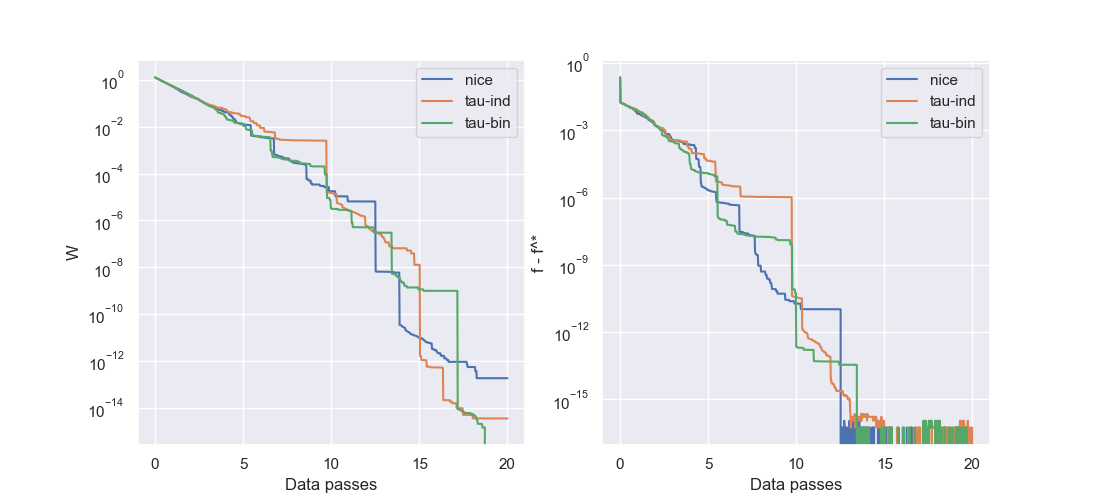
\includegraphics[width=\textwidth]{uniform strategies}
		\caption{Comparison of the $\tau$-nice, $\tau$-independent and $\tau$-binomial strategies}
	\end{figure}
	We see that all the doubly uniform strategies, having the same expected batch size, perform the same convergence rate.
	
	\subsection{Importance Sampling}
	\begin{figure}[h!]\label{fig:2}
		\centering
		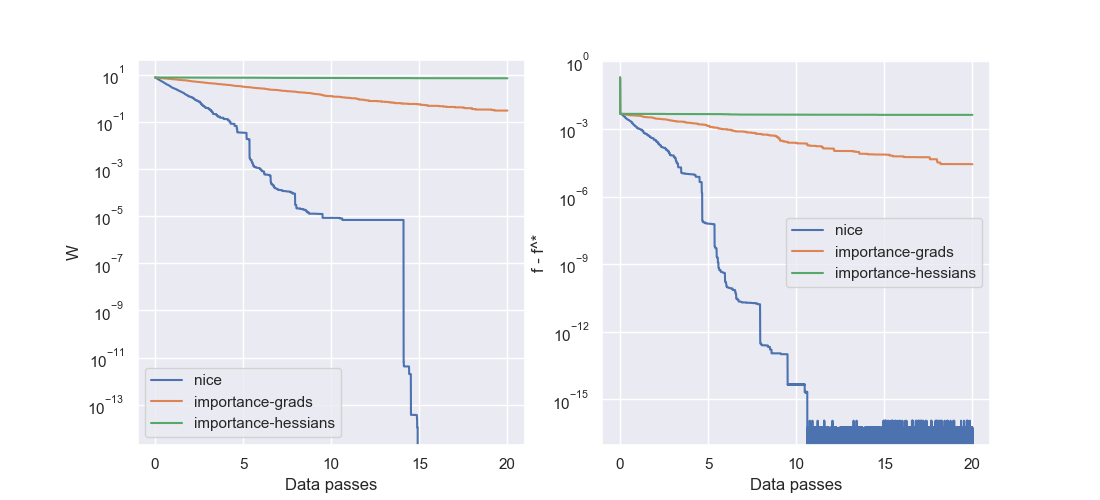
\includegraphics[width=\textwidth]{importance sampling}
		\caption{Comparison of the $\tau$-nice and the Importance Sampling}
	\end{figure}
	We apply both Important Sampling strategies based on Hessians and gradients Lipschitzness parameters. Those are $L_i = \frac{1}{4}\|a_i\|^2$ and $H_i = \frac{1}{10} \|a_i\|^3$ for the logistic regression problem. It is clear that for the considered problem the Importance Sampling used with the Algorithm \ref{SN} does not bring practical improvements.
	
	\subsection{Consecutive strategy}
	\begin{figure}[h!]\label{fig:3}
		\centering
		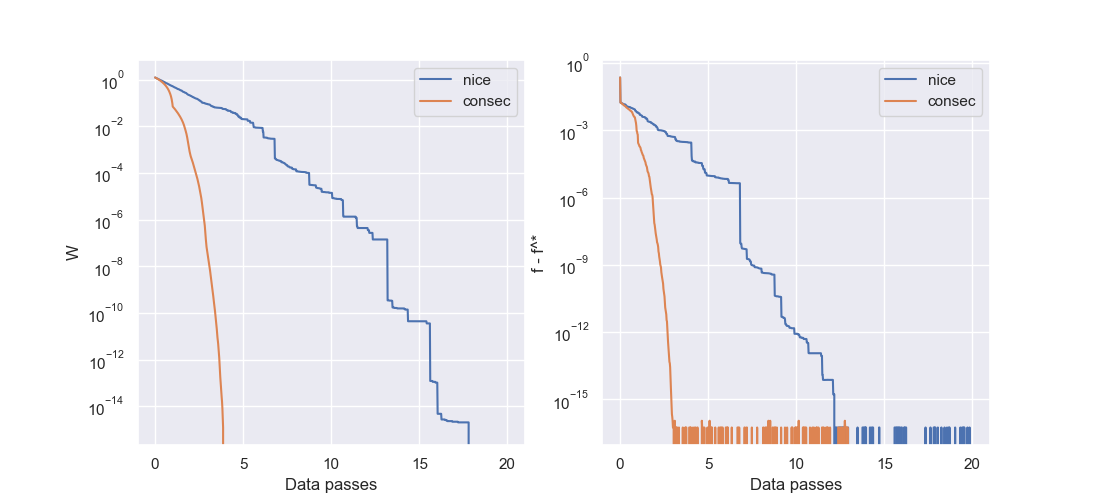
\includegraphics[width=\textwidth]{consecutive strategy 10}
		\caption{Comparison of the $\tau$-nice and the consecutive strategy}
	\end{figure}
	In this case we have a practical improvement. The consecutive strategy does outperform the baseline $\tau$-nice one. Nevertheless, theoretical explainations of this fact are still unclear.
	
	\section{Conclusion}
	So, we do a comparison of different sampling strategies applied to the Stochastic Newton algorithm (\ref{SN}). Firstly, we generalize the linear convergence rate estimations to all Doubly Uniform strategies and determine the practical equivalence of the most common representatives of this type of sampling (Lemma \ref{lemma:4}, Equation \ref{DU convergence}, Figure \ref{fig:1}). Secondly, we obtain that the Importance Sampling is not likely to outperform the usual $\tau$-nice strategy, and has been noticed to be inferior in practice (Figure \ref{fig:2}). Finally, the improvements come from applying the consecutive strategy (Figure \ref{fig:3}). This effect is encouraging, and therefore needs to be studied more precisely.
	
	
	% references title
	\renewcommand\refname{References}	
	\bibliographystyle{plain}
	\bibliography{references}
	
\end{document}
